% SPDX-License-Identifier: LicenseRef-SWARM-NC-Research-1.0 (generated by pandoc 3.6.3 from manuscript.md; do not edit by hand)
% Options for packages loaded elsewhere
\PassOptionsToPackage{unicode}{hyperref}
\PassOptionsToPackage{hyphens}{url}
\documentclass[
]{article}
\usepackage{xcolor}
\usepackage{amsmath,amssymb}
\setcounter{secnumdepth}{-\maxdimen} % remove section numbering
\usepackage{iftex}
\ifPDFTeX
  \usepackage[T1]{fontenc}
  \usepackage[utf8]{inputenc}
  \usepackage{textcomp} % provide euro and other symbols
\else % if luatex or xetex
  \usepackage{unicode-math} % this also loads fontspec
  \defaultfontfeatures{Scale=MatchLowercase}
  \defaultfontfeatures[\rmfamily]{Ligatures=TeX,Scale=1}
\fi
\usepackage{lmodern}
\ifPDFTeX\else
  % xetex/luatex font selection
\fi
% Use upquote if available, for straight quotes in verbatim environments
\IfFileExists{upquote.sty}{\usepackage{upquote}}{}
\IfFileExists{microtype.sty}{% use microtype if available
  \usepackage[]{microtype}
  \UseMicrotypeSet[protrusion]{basicmath} % disable protrusion for tt fonts
}{}
\makeatletter
\@ifundefined{KOMAClassName}{% if non-KOMA class
  \IfFileExists{parskip.sty}{%
    \usepackage{parskip}
  }{% else
    \setlength{\parindent}{0pt}
    \setlength{\parskip}{6pt plus 2pt minus 1pt}}
}{% if KOMA class
  \KOMAoptions{parskip=half}}
\makeatother
\usepackage{longtable,booktabs,array}
\usepackage{calc} % for calculating minipage widths
% Correct order of tables after \paragraph or \subparagraph
\usepackage{etoolbox}
\makeatletter
\patchcmd\longtable{\par}{\if@noskipsec\mbox{}\fi\par}{}{}
\makeatother
% Allow footnotes in longtable head/foot
\IfFileExists{footnotehyper.sty}{\usepackage{footnotehyper}}{\usepackage{footnote}}
\makesavenoteenv{longtable}
\usepackage{graphicx}
\makeatletter
\newsavebox\pandoc@box
\newcommand*\pandocbounded[1]{% scales image to fit in text height/width
  \sbox\pandoc@box{#1}%
  \Gscale@div\@tempa{\textheight}{\dimexpr\ht\pandoc@box+\dp\pandoc@box\relax}%
  \Gscale@div\@tempb{\linewidth}{\wd\pandoc@box}%
  \ifdim\@tempb\p@<\@tempa\p@\let\@tempa\@tempb\fi% select the smaller of both
  \ifdim\@tempa\p@<\p@\scalebox{\@tempa}{\usebox\pandoc@box}%
  \else\usebox{\pandoc@box}%
  \fi%
}
% Set default figure placement to htbp
\def\fps@figure{htbp}
\makeatother
\setlength{\emergencystretch}{3em} % prevent overfull lines
\providecommand{\tightlist}{%
  \setlength{\itemsep}{0pt}\setlength{\parskip}{0pt}}
\usepackage{bookmark}
\IfFileExists{xurl.sty}{\usepackage{xurl}}{} % add URL line breaks if available
\urlstyle{same}
\hypersetup{
  pdftitle={A zonal separation-cohesion rule sustains less order than alignment alone, and the design did not measure recovery: a preregistered simulation comparison under a heading shock},
  pdfauthor={Mohamed Bechir Kefi, independent researcher},
  hidelinks,
  pdfcreator={LaTeX via pandoc}}

\title{A zonal separation-cohesion rule sustains less order than
alignment alone, and the design did not measure recovery: a
preregistered simulation comparison under a heading shock}
\usepackage{etoolbox}
\makeatletter
\providecommand{\subtitle}[1]{% add subtitle to \maketitle
  \apptocmd{\@title}{\par {\large #1 \par}}{}{}
}
\makeatother
\subtitle{Independent research manuscript / preprint draft, not
peer-reviewed. All results are simulated.}
\author{Mohamed Bechir Kefi, independent researcher}
\date{Draft of 2026-11-25 (M6 release candidate)}

\begin{document}
\maketitle

\section{Abstract}\label{abstract}

Local interaction rules in self-propelled particle models are often
described as producing coordinated motion without a leader, but it is
less clear how adding separation and cohesion to pure alignment changes
a group's response to a disturbance. We compared, in a two-dimensional
simulation with 200 agents, an alignment-only rule (A0), a zonal rule
with separation, alignment and cohesion (A1, cohesion weight 0.5) and a
centralized global-alignment reference (A2). Half the agents received
random headings after 3,000 steps. The protocol, analysis code and seeds
were frozen before the confirmatory runs. Across 18 cells of density,
noise and radius with 20 matched seeds each (1,080 runs, none failed),
the primary contrast in mean post-disturbance polarization was Delta =
-0.307 (95\% stratified bootstrap CI {[}-0.313, -0.302{]}), which
rejects the null hypothesis under the frozen rule. The same gap was
present before the shock (-0.312 {[}-0.319, -0.304{]}): A1 was weakly
ordered in every cell (mean pre-shock polarization 0.097 to 0.229). Four
frozen sensitivity conditions (topological neighbours, cohesion weights
0.25 and 1.0, reflecting walls; 480 runs) kept the sign and excluded
zero. An exploratory change-score analysis, made after the results were
seen, gave 0.004 {[}-0.004, 0.012{]}. The confirmatory result is
therefore a robust difference in sustained pre-shock order at this
parameterisation, not evidence that separation and cohesion impair or
improve recovery. The design could not measure A1's recovery of order.
These are statements about a simulated model in the tested grid only.

\section{Keywords}\label{keywords}

collective motion; Vicsek model; zonal flocking rules; disturbance
recovery; preregistered simulation; negative result

\section{1. Introduction}\label{introduction}

Models of collective motion show that agents following purely local
rules can move in a common direction without any leader or global
signal. The alignment-only model of Vicsek et al.~(1995) produces a
transition from disordered to ordered motion as noise falls or density
rises. Zonal models add short-range repulsion and longer-range
attraction to alignment (Reynolds, 1987; Couzin et al., 2002), and
control-theoretic flocking algorithms combine alignment, separation and
cohesion terms (Olfati-Saber, 2006). A natural engineering and modelling
question follows: when a group is disturbed, do the extra separation and
cohesion terms help it regain order, for example by keeping
neighbourhoods connected, or do they hurt, because repulsion introduces
direction changes unrelated to heading?

This manuscript reports a small preregistered simulation study of that
question. The research question, from the project's master prompt, is:
\emph{how do local interaction rules affect collective coordination
under disturbances?} We operationalised it as a paired comparison of
mean polarization after a heading shock between A1 (separation,
alignment and cohesion) and A0 (alignment only), with a centralized
reference A2, under matched initial conditions, noise and disturbance.

\textbf{Hypotheses.} H0: the pooled mean paired difference Delta in
post-disturbance polarization between A1 and A0 is zero. H1
(nondirectional): Delta is not zero. The smallest effect size of
interest (SESOI) was 0.05 polarization units.

\textbf{Contributions.} The contributions are deliberately narrow:

\begin{enumerate}
\def\labelenumi{\arabic{enumi}.}
\tightlist
\item
  A frozen, hash-recorded protocol and analysis for a matched-seed
  comparison of alignment-only and zonal rules under a defined heading
  shock, with a centralized reference and seed-level uncertainty
  (EXP-002, 1,080 runs).
\item
  A frozen sensitivity experiment that varies neighbourhood type,
  cohesion weight and boundary (EXP-003, 480 runs).
\item
  A documented negative finding about the design: the primary outcome
  measured a difference in sustained order between the rules rather than
  recovery, a risk that was anticipated before the freeze and then
  realised. We report it as the main result rather than reinterpreting
  the outcome.
\item
  A reproducible implementation with verification tests and complete
  provenance for every run.
\end{enumerate}

No novelty is claimed: the literature review was targeted, not
systematic.

\section{2. Related work}\label{related-work}

All sources below were checked for bibliographic metadata
(\texttt{research/literature\_review.md}). In M6 (2026-11-25), a free
legal full text was consulted for seven of the eight sources to check
the specific statement made about each, and the page or section is
recorded in \texttt{research/publication/evidence\_audit.md}; the
reference list states, for each source, which version was consulted and
how much of it. Couzin et al.~(2002) remains read at the abstract level
only. Statements about the sources are limited to what was checked.

\textbf{Alignment-only models.} Vicsek et al.~(1995) introduced
self-driven particles that adopt the mean heading of neighbours within a
radius plus noise, and reported a noise- and density-driven transition
to ordered motion. Our A0 is this rule. Vicsek and Zafeiris (2012)
review this family of models and their order parameters.

\textbf{Zonal and steering-rule models.} Reynolds (1987) proposed
separation, alignment and cohesion steering rules for animated flocks.
Couzin et al.~(2002) studied a model with zones of repulsion,
orientation and attraction and reported that changes in zone sizes shift
the collective state and that the system shows history dependence. Our
A1 uses the zonal priority of that model (repulsion first), with fixed
weights.

\textbf{Control-theoretic flocking.} Jadbabaie, Lin and Morse (2003)
studied the coordination of groups of mobile autonomous agents using
nearest-neighbour rules; its full text was consulted only to confirm the
topic, so we cite it for its topic and do not characterise its results.
Olfati-Saber (2006) presented flocking algorithms with alignment,
separation and cohesion and stated that flocks need no leaders. Cucker
and Smale (2007) studied velocity consensus with distance-decaying
coupling. Cucker and Smale (2007; Theorem 1 of the authors' preprint)
relate convergence to how coupling decays with distance between agents;
this, together with the cohesion terms of Olfati-Saber (2006), motivated
the mechanism in H1 that cohesion may preserve connectivity and so help
recovery. None of these sources tests our specific disturbance.

\textbf{Neighbourhood type.} Ballerini et al.~(2008) reported field
evidence that starlings interact with a fixed number of neighbours
(about six to seven) rather than all neighbours within a fixed distance.
This motivated our topological sensitivity condition. We make no claim
of biological fidelity.

\textbf{Relation of this work.} The study is an application of known
models, not an extension of their theory. What it adds is a controlled,
preregistered paired comparison under one disturbance, together with a
clear account of why its primary outcome did not isolate recovery. We
did not find, in the sources read, a matched comparison of exactly this
kind, but the review was not systematic and we do not claim that none
exists.

\section{3. Background and formal
model}\label{background-and-formal-model}

\textbf{Agents and space.} \(N = 200\) agents move in a square box of
side \(L\) with positions \(x_i \in \mathbb{R}^2\) (length unit u) and
headings \(\theta_i \in (-\pi, \pi]\), at constant speed \(v_0 = 0.05\)
u per step. Time is discrete and updates are synchronous. The primary
boundary is periodic; density is \(\rho = N / L^2\).

\textbf{Neighbourhoods.} Metric:
\(\mathcal{N}_i(t) = \{ j \neq i : \lVert x_j - x_i \rVert \le r \}\),
with torus distance. The topological alternative (EXP-003 S1) uses the
\(k = 7\) nearest agents.

\textbf{Noise.} Each step,
\(\xi_i(t) \sim \mathrm{Uniform}(-\eta\pi, \eta\pi)\).

\textbf{Arms.}

\begin{itemize}
\tightlist
\item
  A0 (alignment only, baseline):
  \(\theta_i(t+1) = \arg \sum_{j \in \mathcal{N}_i \cup \{i\}} e^{\mathrm{i}\theta_j(t)} + \xi_i(t)\).
\item
  A1 (separation, alignment, cohesion): with \(a_i\) the unit mean
  neighbour heading (self included), \(s_i\) the unit repulsion vector
  from neighbours within \(r_s = 0.25 r\), and \(c_i\) the unit vector
  to the neighbour centroid, the desired direction is \(d_i = s_i\) if
  any neighbour lies within \(r_s\), and \(d_i = w_a a_i + w_c c_i\)
  otherwise, with \(w_a = 1\) and \(w_c = 0.5\). Then
  \(\theta_i(t+1) = \arg d_i + \xi_i(t)\). With \(r_s = 0\) and
  \(w_c = 0\), A1 reduces exactly to A0 (tested).
\item
  A2 (centralized reference): every agent adopts the global mean heading
  of all \(N\) agents plus the same noise. It is an idealised broadcast
  ceiling, not a candidate local rule.
\end{itemize}

\textbf{Disturbance.} At step \(t_d = 3000\), a fraction \(f = 0.5\) of
agents, chosen by the run's disturbance random stream, receive headings
drawn uniformly on \((-\pi, \pi]\). For a given seed, the same agents
receive the same new headings in every arm (common random numbers).

\textbf{Order parameter.}
\(\varphi(t) = \lvert N^{-1} \sum_i e^{\mathrm{i}\theta_i(t)} \rvert \in [0, 1]\).
Primary outcome: \(\varphi_{\text{post}}\), the mean of \(\varphi(t)\)
over \(t \in [t_d, t_d + W)\) with \(W = 500\). Pre-shock level:
\(\varphi_{\text{pre}}\), the mean over \([t_d - 100, t_d)\). For \(N\)
independent uniform headings the expected value of \(\varphi\) is about
\(\sqrt{\pi} / (2\sqrt{N}) \approx 0.063\) (used only in the exploratory
check X4); the EXP-001 planning summary uses the root-mean-square value
\(1/\sqrt{N} \approx 0.071\) as its reference. Both describe the same
random level.

\textbf{Estimand.}
\(\Delta = \frac{1}{18} \sum_{c} \frac{1}{20} \sum_{s} \left[ \varphi_{\text{post}}(A1, c, s) - \varphi_{\text{post}}(A0, c, s) \right]\),
the equal-weight mean over cells \(c\) of the within-cell mean paired
difference over seeds \(s\).

\textbf{Secondary metrics.} Recovery time \(\tau\): the first step
\(t \ge t_d\) from which \(\varphi \ge 0.9\,\varphi_{\text{pre}}\) holds
for 10 steps, right-censored at \(W\). Cohesion \(C\): the fraction of
agents in the largest connected component of the radius-\(r\) graph,
averaged over the post window. Collisions: pairs closer than \(0.1 r\),
per agent per 100 steps. Neighbour cost: pair-distance evaluations per
step (deterministic) and wall-clock time per step.

\textbf{Complexity.} Neighbour search uses a cell list, whose distance
evaluations depend on local density, verified against a brute-force
reference that evaluates all \(N(N-1)/2 = 19{,}900\) pairs per step.

\section{4. Methods}\label{methods}

\subsection{4.1 Design and protocol
registration}\label{design-and-protocol-registration}

Three experiments were registered
(\texttt{research/experiment\_registry.csv}). EXP-001 is exploratory by
design: implementation verification, a 15-run smoke matrix and planning
scans. EXP-002 (primary) and EXP-003 (sensitivity) are confirmatory.
Their protocols and configurations were frozen by the owner on
2026-11-24 as protocol v1.0; SHA-256 hashes of the three protocol files
and four configurations and the git revision are in
\texttt{research/protocol\_freeze.json}. The runner refuses any
confirmatory configuration whose canonical hash is not in that record.

Four owner-approved amendments were applied before the freeze, prompted
by exploratory EXP-001 scans (AM-1 to AM-4;
\texttt{research/protocol.md} section 13): (AM-1) the A1 cohesion weight
was set by the owner to 0.5 (draft 1.0, at which A1 never ordered in the
scans), without tuning on the contrast; (AM-2) the burn-in was
lengthened by a rule R-BI written and committed before its data existed,
giving \(t_d = 3000\); (AM-3) 20 seeds instead of 10; (AM-4) budget caps
kept. Rule R-BI used A0-only runs without a shock (seeds 321 to 325) and
selected the smallest candidate burn-in at which A0 was aligned (mean
\(\varphi \ge 0.5\)) in every cell where it could align at all. A0 could
align in 8 of 18 cells; the other 10 were kept in the estimand and
flagged.

\textbf{Disclosure.} Primary-outcome values from one smoke cell under
the draft design were seen before the freeze (A1 - A0 mean
\(\varphi_{\text{post}}\) -0.480, SD 0.059, 5 seeds; recorded in the
freeze record). The confirmatory design differs from the draft (cohesion
weight, burn-in, seeds), but the direction of the draft smoke contrast
was known.

\subsection{4.2 Simulation matrix}\label{simulation-matrix}

EXP-002: arms A0, A1, A2; density \(\rho \in \{0.5, 1, 2\}\); noise
\(\eta \in \{0.1, 0.3, 0.5\}\); radius \(r \in \{0.5, 1\}\); seeds 1001
to 1020, the same in every arm; \(T = 3500\). That is
\(3 \times 18 \times 20 = 1080\) runs. A seed fixes the initial state,
the per-step noise stream and the disturbance draw for all arms.

EXP-003: A0 and A1 on four reduced cells (\(\rho \in \{0.5, 2\}\),
\(\eta \in \{0.1, 0.5\}\), \(r = 1\)), seeds 1001 to 1020, one change at
a time: S1 topological \(k = 7\); S2a and S2b \(w_c = 0.25\) and \(1.0\)
(A1 only, paired with the EXP-002 A0 runs of the same cell and seed); S3
reflecting walls; S4 recovery thresholds 0.8 and 0.95, computed from the
stored EXP-002 series. The configurations hold 480 runs.

\subsection{4.3 Statistical analysis}\label{statistical-analysis}

The independent unit is the (cell, seed) pair; time steps are never
treated as independent. Uncertainty is a stratified percentile
bootstrap: seeds are resampled with replacement within each cell, 10,000
resamples, seed 20261124, 95\% CI. The CI is conditional on the 18
tested cells and their equal weights; it describes seed-to-seed
variation within those cells, not uncertainty over other densities,
noises or radii. Decision rule (frozen): if the CI excludes 0, H0 is
rejected; if it lies inside (-0.05, 0.05), the result is practically
equivalent; otherwise it is inconclusive. Per-cell differences and all
secondary metrics are descriptive, with CIs and no per-cell tests. For
EXP-003, a condition invalidates the EXP-002 interpretation if its CI
lies entirely on the opposite side of zero from the EXP-002 estimate,
and weakens it if its CI contains zero while the EXP-002 CI does not. A
run could be excluded only for a software failure; more than 5\%
failures in an arm would stop the analysis. The analysis script
\texttt{experiments/analyse\_confirmatory.py} was committed (revision
\texttt{075cf7c}) before any confirmatory output existed; its one
interpretive choice (which EXP-002 reference EXP-003 is classified
against) was fixed in writing beforehand (decision DL-012).

\textbf{Exploratory analyses.} After seeing the confirmatory results, we
computed five further quantities from the same committed runs, without
new simulation (\texttt{experiments/exploratory\_m4.py}, journal
EXPL-M4-01): X1 the paired change score
\((\varphi_{\text{post}} - \varphi_{\text{pre}})\); X2 the primary
contrast split by whether A0 can align in a cell; X3 the contrast in
cells where the two arms' mean pre-shock order differs by less than the
SESOI; X4 the early response over \([t_d, t_d + 50)\); X5 the change
score for each EXP-003 condition. They use the frozen bootstrap
settings, are labelled exploratory throughout, and do not alter any
frozen verdict.

\subsection{4.4 Implementation and
verification}\label{implementation-and-verification}

The simulator is a Python package (\texttt{src/swarm/}) with numpy.
Verification (EXP-001): the cell list and brute-force neighbour search
agreed on every step of a 72-row benchmark (0 mismatched steps);
repeated runs are bit-identical; bounds on headings, \(\varphi\),
cohesion and positions hold; hand-computed two- and three-agent examples
match the update rules; A1 reduces to A0 when its extra terms are
switched off. The test suite passed with 133 tests at the confirmatory
revision. During each confirmatory analysis, \(\varphi_{\text{pre}}\),
\(\varphi_{\text{post}}\) and \(\tau\) were recomputed from every stored
series: 1,080 of 1,080 EXP-002 runs and 160 of 160 runs per EXP-003
condition matched, with 0 mismatches.

\subsection{4.5 Resources and
provenance}\label{resources-and-provenance}

Runs used an Apple M1 Pro (10 cores, 16 GB), macOS 15.3.1, Python 3.12.1
and numpy 2.5.4, with 2 worker processes under \texttt{nice}. EXP-002
took 1138.7 s of wall-clock time against a 4-hour budget; EXP-003 took
594.7 s (S1), 181.9 s (S2) and 293.9 s (S3) against 2 hours. Unrelated
processes loaded the machine heavily during the runs (the 15-minute load
average recorded at the EXP-003 S1 launch was 38.7), so wall-clock
figures are inflated and only indicative. Every run records its
configuration hash, seed, code revision, data-manifest hash, hardware
and times (\texttt{provenance.csv}), and every raw file has a SHA-256
entry (\texttt{raw\_manifest.json}); all 1,584 listed files were
re-hashed in M4 with 0 mismatches.

\textbf{Deviations.} (1) 2 worker processes were used instead of the 8
in the protocols' example commands; each run is single-threaded and
seeded, so outputs cannot change. (2) 454 EXP-003 runs record an
uncommitted working tree because a journal file was edited during the
runs; no code, configuration or protocol differed from \texttt{075cf7c},
and 6 flagged runs re-simulated from clean code were bit-identical
(DL-013). (3) The standalone experiment reports were written after M3
from committed results, on the owner's approval (DL-014). No run failed
and none was excluded.

\section{5. Results}\label{results}

\subsection{5.1 EXP-001: verification and planning
(exploratory)}\label{exp-001-verification-and-planning-exploratory}

All verification checks passed. The planning scans showed that A1 never
ordered at the draft cohesion weight \(w_c = 1\) (mean
\(\varphi_{\text{pre}}\) 0.057 to 0.071 in all 18 cells, close to the
random level) and that A0 was disordered before the shock in many cells.
These findings led to the amendments in Section 4.1. The seed spread of
the paired \(\varphi_{\text{post}}\) difference in the smoke cell was
0.059, below the 0.2 assumed in the sample-size plan.

\subsection{5.2 EXP-002: primary comparison
(confirmatory)}\label{exp-002-primary-comparison-confirmatory}

All 1,080 runs completed; none failed or was excluded; every cell has 20
pairs.

\textbf{Table 1.} Pooled contrasts in EXP-002 (360 (cell, seed) pairs;
stratified bootstrap 95\% CIs). Source:
\texttt{results/confirmatory/EXP-002/analysis/analysis.json}.

\begin{longtable}[]{@{}
  >{\raggedright\arraybackslash}p{(\linewidth - 4\tabcolsep) * \real{0.3333}}
  >{\raggedright\arraybackslash}p{(\linewidth - 4\tabcolsep) * \real{0.3333}}
  >{\raggedright\arraybackslash}p{(\linewidth - 4\tabcolsep) * \real{0.3333}}@{}}
\toprule\noalign{}
\begin{minipage}[b]{\linewidth}\raggedright
quantity
\end{minipage} & \begin{minipage}[b]{\linewidth}\raggedright
estimate {[}95\% CI{]}
\end{minipage} & \begin{minipage}[b]{\linewidth}\raggedright
status
\end{minipage} \\
\midrule\noalign{}
\endhead
\bottomrule\noalign{}
\endlastfoot
Delta = A1 - A0, phi\_post (primary) & -0.307 {[}-0.313, -0.302{]} &
rejects H0 (frozen rule) \\
A1 - A0, phi\_pre & -0.312 {[}-0.319, -0.304{]} & descriptive \\
A2 - A0, phi\_post & 0.374 {[}0.369, 0.379{]} & descriptive
(reference) \\
A2 - A1, phi\_post & 0.681 {[}0.679, 0.684{]} & descriptive
(reference) \\
A1 - A0, cohesion C & 0.080 {[}0.065, 0.094{]} & descriptive \\
A1 - A0, collisions per agent per 100 steps & -2.951 {[}-3.027,
-2.874{]} & descriptive \\
A2 - A0, cohesion C & -0.210 {[}-0.218, -0.202{]} & descriptive \\
A2 - A0, collisions per agent per 100 steps & -2.174 {[}-2.258,
-2.089{]} & descriptive \\
\end{longtable}

The primary CI excludes zero and lies far outside the SESOI band, so H0
is rejected. The direction is negative: A1 is less polarized than A0
after the shock.

\textbf{The pre-shock gap.} A1 was weakly ordered before the shock in
every cell: its cell-mean \(\varphi_{\text{pre}}\) ranged from 0.097 to
0.229. The pooled pre-shock gap, -0.312 {[}-0.319, -0.304{]}, is as
large as Delta. In the per-cell table, \(\varphi_{\text{post}}\) is
close to \(\varphi_{\text{pre}}\) for every arm in every cell
(supplementary Table S2).

\textbf{Per-cell heterogeneity.} The per-cell mean differences range
from -0.810 to +0.037. In the 8 cells where A0 aligns, they range from
-0.406 to -0.810. In the 10 flagged cells, where A0 is also disordered,
they are small and of either sign, for example +0.037 {[}0.029, 0.044{]}
at \(\rho = 0.5\), \(\eta = 0.3\), \(r = 0.5\) and -0.001 {[}-0.007,
0.004{]} at \(\rho = 0.5\), \(\eta = 0.5\), \(r = 1\). Figure 1 shows
all cells.

\begin{figure}
\centering
\pandocbounded{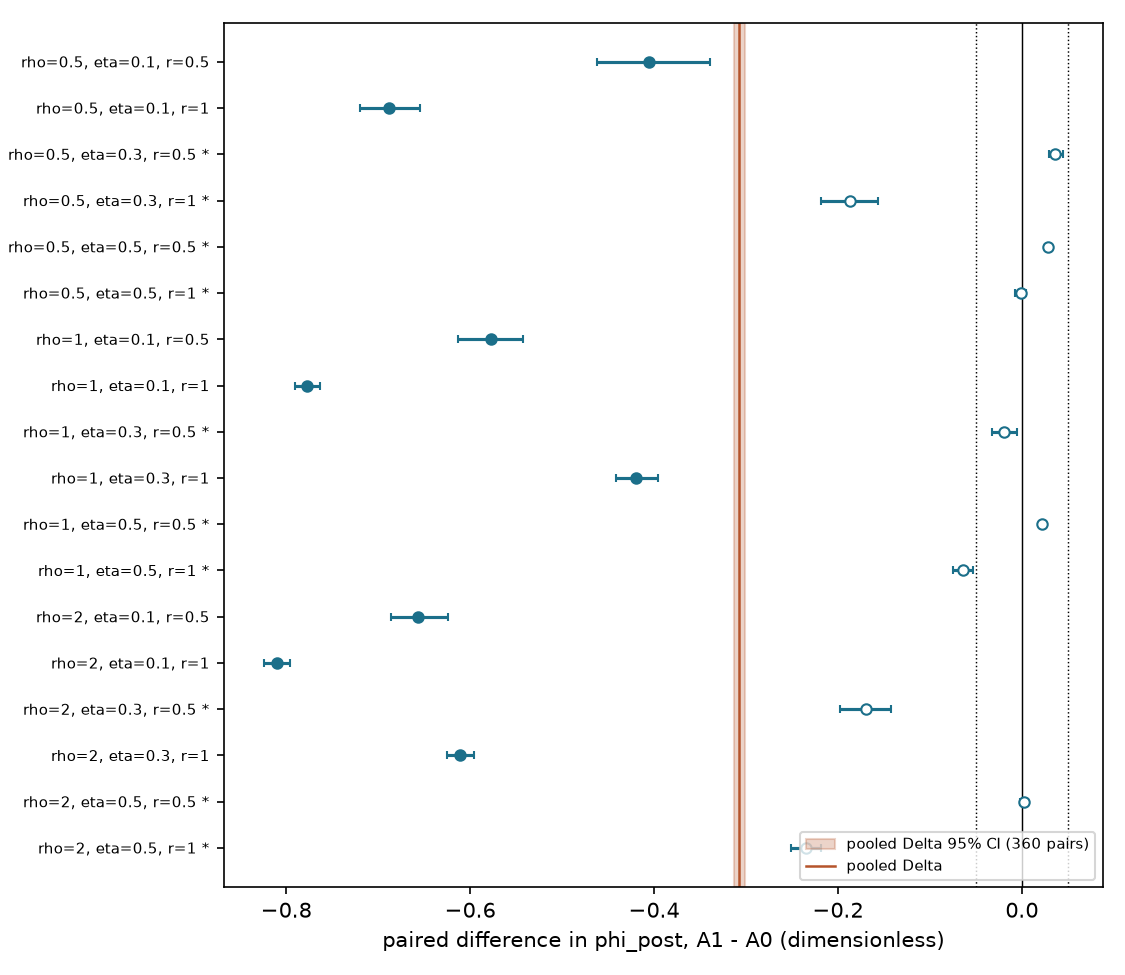
\includegraphics[keepaspectratio]{../../results/confirmatory/EXP-002/analysis/fig_exp002_01_forest.png}}
\caption{Figure 1 (FIG-EXP002-01). Per-cell mean paired difference
phi\_post(A1) - phi\_post(A0) with 95\% stratified-bootstrap CIs (20
seeds per cell; 10,000 resamples). Shaded band and solid line: pooled
Delta and its CI. Dotted lines: SESOI +/- 0.05. Hollow markers and *
mark the 10 cells where A0 is not aligned before the shock (rule R-BI).
Simulated data, confirmatory. Alt text: a forest plot in which most
cells lie well below zero, the 8 ordered cells furthest below, and the
high-noise cells near zero.}
\end{figure}

\textbf{Time course.} Figure 2 shows mean \(\varphi(t)\) from step 2800
to 3499. A0 dips at the shock and returns within tens of steps in
ordered cells; A1 stays at \(\varphi\) of about 0.1 to 0.2 throughout.
The A0 median recovery time at the 0.9 threshold was 1.0 to 10.5 steps
in the 8 cells where A0 aligns. A2 recovered in one step in every cell,
by construction.

\begin{figure}
\centering
\pandocbounded{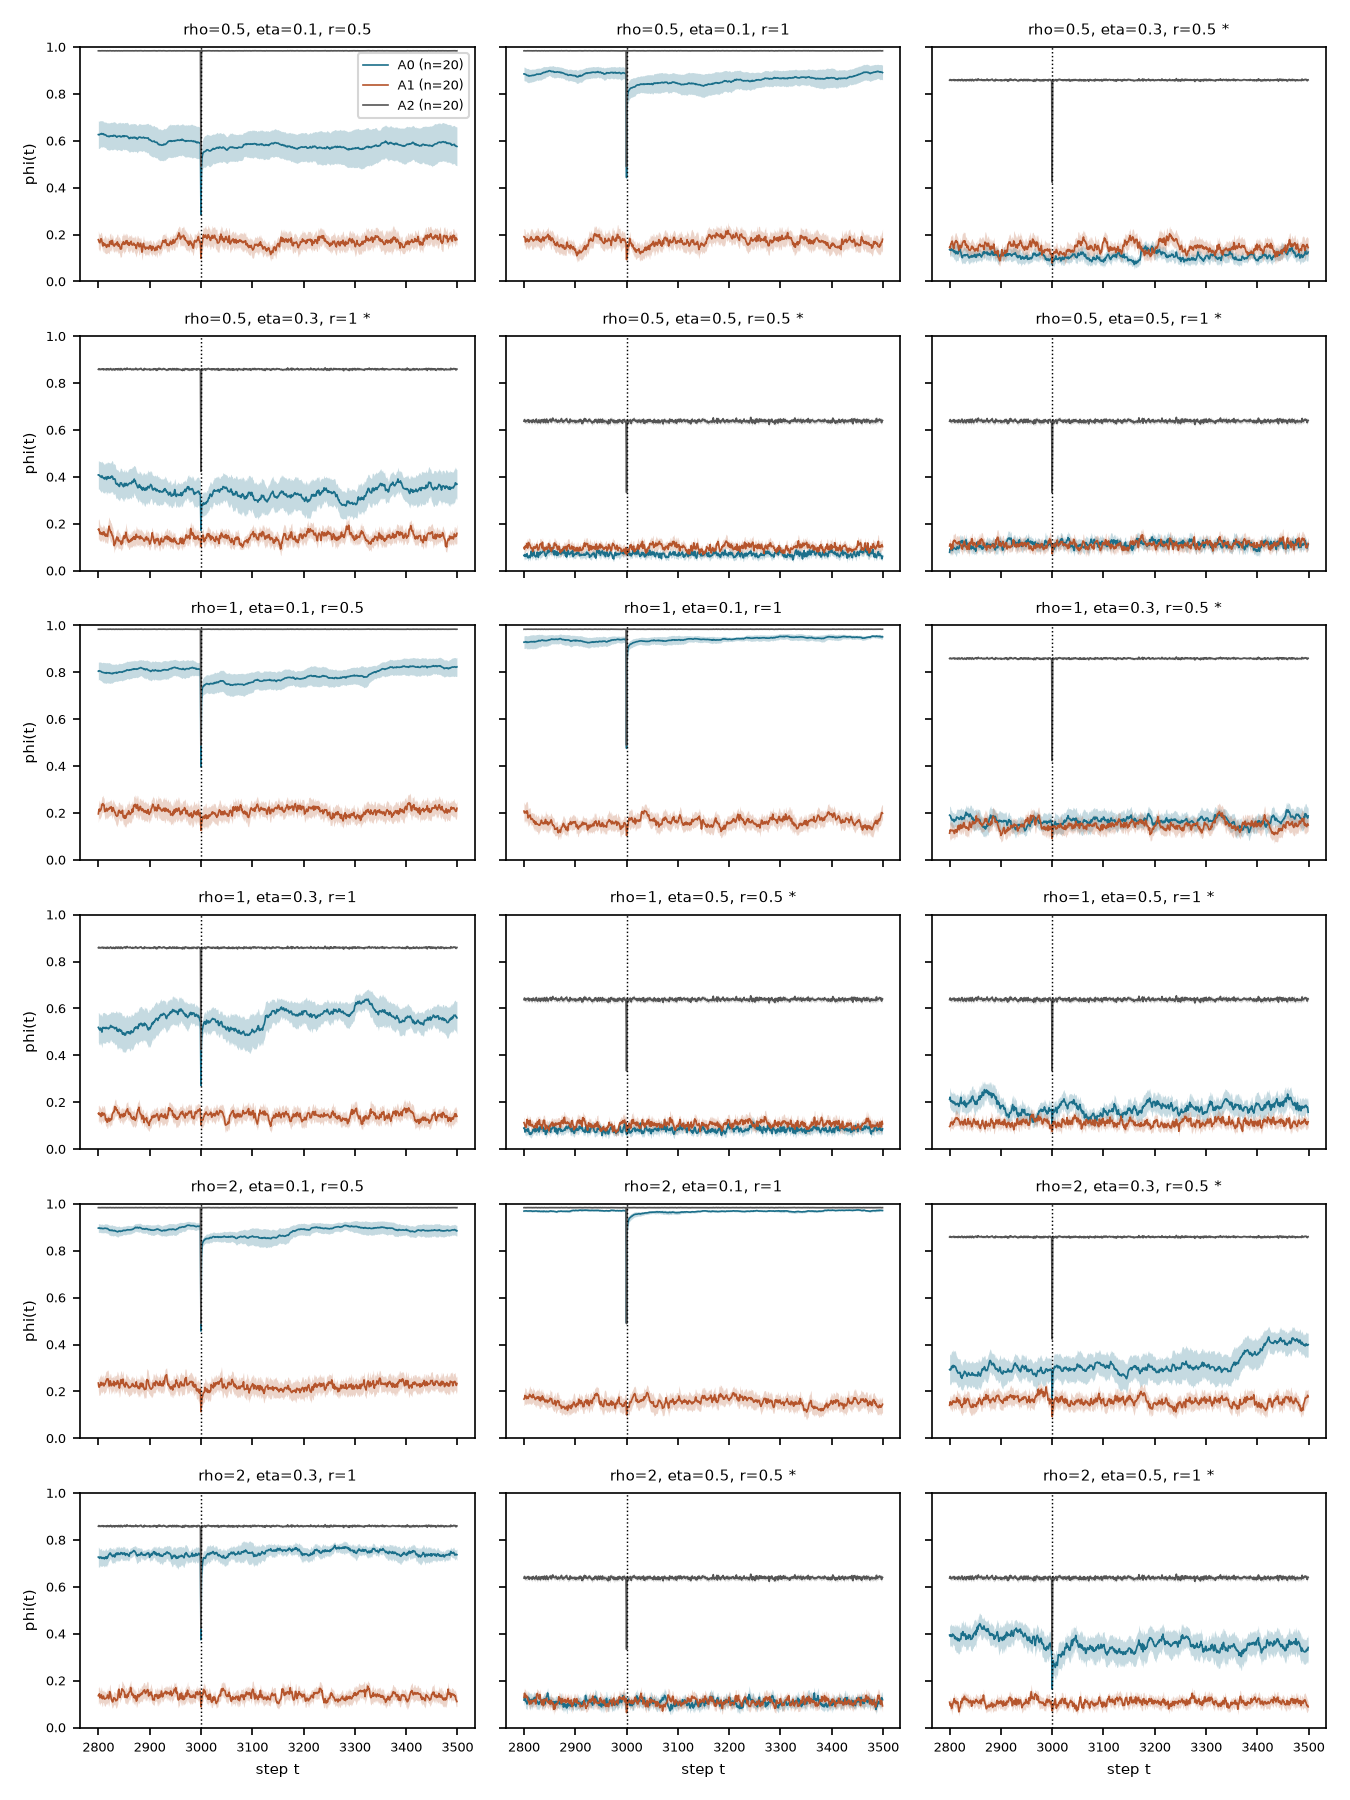
\includegraphics[keepaspectratio]{../../results/confirmatory/EXP-002/analysis/fig_exp002_02_timeseries.png}}
\caption{Figure 2 (FIG-EXP002-02). Mean polarization phi(t) across 20
seeds per arm, steps 2800 to 3499, with a band of +/- 1.96 standard
errors across seeds; dotted line: shock at t\_d = 3000. * marks cells
where A0 is not orderable (rule R-BI). Simulated data, confirmatory. Alt
text: small multiples, one per cell; A2 near the top, A0 high in
low-noise cells with a brief dip at the shock, A1 low and flat.}
\end{figure}

\textbf{Secondary metrics.} A1 had higher post-window cohesion than A0
(0.080 {[}0.065, 0.094{]}) and fewer collisions (-2.951 {[}-3.027,
-2.874{]} per agent per 100 steps). Higher connectivity did not come
with higher alignment. A1 required more pair-distance evaluations per
step than A0 in every cell (for example 8087 against 3562 at
\(\rho = 2\), \(\eta = 0.1\), \(r = 1\)), consistent with its agents
clustering more tightly; A2 required fewer than A0 in every cell (2203
in the same cell). All counts stay below the 19,900 pairs of brute
force. Recovery times are in supplementary Table S3; they are relative
to each arm's own \(\varphi_{\text{pre}}\), so A1's \(\tau\) measures a
return to a disordered level and is not comparable with A0's.

\subsection{5.3 EXP-003: sensitivity
(confirmatory)}\label{exp-003-sensitivity-confirmatory}

All 480 runs completed with no failures.

\textbf{Table 2.} Delta\_S per sensitivity condition on the four reduced
cells (80 pairs each). Source:
\texttt{results/confirmatory/EXP-003-analysis/analysis.json}.

\begin{longtable}[]{@{}
  >{\raggedright\arraybackslash}p{(\linewidth - 6\tabcolsep) * \real{0.2500}}
  >{\raggedright\arraybackslash}p{(\linewidth - 6\tabcolsep) * \real{0.2500}}
  >{\raggedright\arraybackslash}p{(\linewidth - 6\tabcolsep) * \real{0.2500}}
  >{\raggedright\arraybackslash}p{(\linewidth - 6\tabcolsep) * \real{0.2500}}@{}}
\toprule\noalign{}
\begin{minipage}[b]{\linewidth}\raggedright
condition
\end{minipage} & \begin{minipage}[b]{\linewidth}\raggedright
Delta\_S {[}95\% CI{]}
\end{minipage} & \begin{minipage}[b]{\linewidth}\raggedright
verdict against pooled EXP-002
\end{minipage} & \begin{minipage}[b]{\linewidth}\raggedright
verdict against EXP-002 on the 4 cells
\end{minipage} \\
\midrule\noalign{}
\endhead
\bottomrule\noalign{}
\endlastfoot
EXP-002, 18 cells (reference) & -0.307 {[}-0.313, -0.302{]} & & \\
EXP-002, 4 reduced cells (reference) & -0.434 {[}-0.443, -0.424{]} &
& \\
S1 topological k = 7 & -0.415 {[}-0.429, -0.398{]} & neither invalidated
nor weakened & neither \\
S2a w\_c = 0.25 & -0.268 {[}-0.282, -0.257{]} & neither & neither \\
S2b w\_c = 1.0 & -0.507 {[}-0.515, -0.498{]} & neither & neither \\
S3 reflecting walls & -0.449 {[}-0.463, -0.434{]} & neither & neither \\
\end{longtable}

No condition invalidates or weakens the EXP-002 result. The magnitude
increases with the cohesion weight: -0.268 at 0.25, -0.434 at 0.5
(EXP-002 on the same cells) and -0.507 at 1.0. The pre-shock gap again
matches the post-shock contrast where it was computed: -0.438 {[}-0.454,
-0.422{]} in S1 and -0.434 {[}-0.460, -0.405{]} in S3. Some high-noise
cells have near-zero or positive per-cell differences (S2a +0.053 and S3
-0.003 at \(\rho = 0.5\), \(\eta = 0.5\)). S4 recovery-time medians rise
with the threshold, with at most 3 of 20 runs censored in any arm and
cell.

\begin{figure}
\centering
\pandocbounded{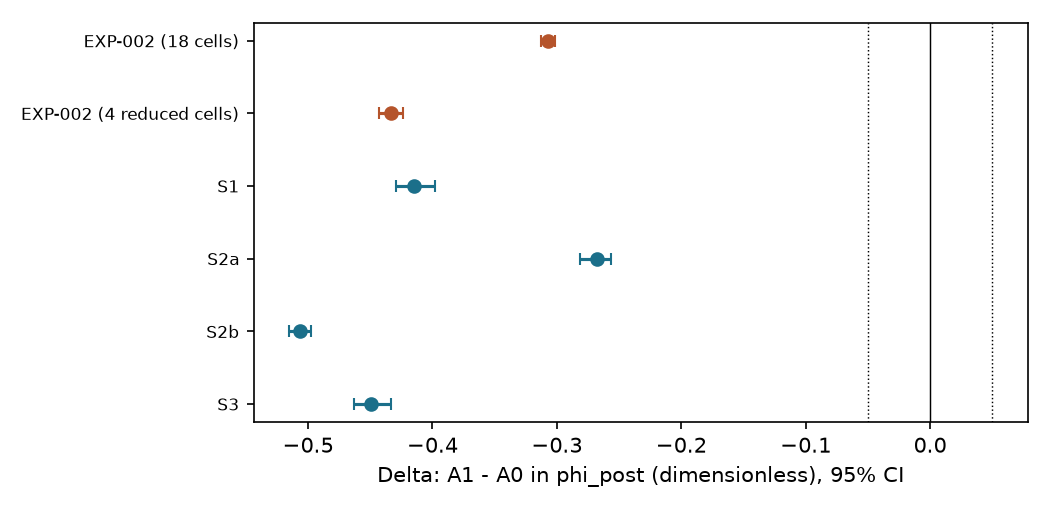
\includegraphics[keepaspectratio]{../../results/confirmatory/EXP-003-analysis/fig_exp003_01_sensitivity.png}}
\caption{Figure 3 (FIG-EXP003-01). Delta (A1 - A0 in phi\_post) with
95\% stratified-bootstrap CIs (20 seeds per cell, 10,000 resamples) for
EXP-002 (all 18 cells and the 4 reduced cells) and each EXP-003
condition. Dotted lines: SESOI +/- 0.05. Simulated data, confirmatory.
Alt text: six intervals, all far below zero and below the SESOI band.}
\end{figure}

\subsection{5.4 Exploratory checks of the pre-shock
confound}\label{exploratory-checks-of-the-pre-shock-confound}

These analyses were made after the confirmatory results were seen and
are exploratory.

\textbf{Table 3.} Exploratory contrasts A1 - A0 (frozen bootstrap
settings). Source:
\texttt{results/exploratory/M4-sensitivity/analysis.json}.

\begin{longtable}[]{@{}
  >{\raggedright\arraybackslash}p{(\linewidth - 6\tabcolsep) * \real{0.2500}}
  >{\raggedright\arraybackslash}p{(\linewidth - 6\tabcolsep) * \real{0.2500}}
  >{\raggedright\arraybackslash}p{(\linewidth - 6\tabcolsep) * \real{0.2500}}
  >{\raggedright\arraybackslash}p{(\linewidth - 6\tabcolsep) * \real{0.2500}}@{}}
\toprule\noalign{}
\begin{minipage}[b]{\linewidth}\raggedright
id
\end{minipage} & \begin{minipage}[b]{\linewidth}\raggedright
quantity
\end{minipage} & \begin{minipage}[b]{\linewidth}\raggedright
cells / pairs
\end{minipage} & \begin{minipage}[b]{\linewidth}\raggedright
estimate {[}95\% CI{]}
\end{minipage} \\
\midrule\noalign{}
\endhead
\bottomrule\noalign{}
\endlastfoot
X1 & change score phi\_post - phi\_pre, all cells & 18 / 360 & 0.004
{[}-0.004, 0.012{]} \\
X1 & change score, 8 cells where A0 aligns & 8 / 160 & 0.012 {[}-0.002,
0.026{]} \\
X2 & phi\_post, 8 cells where A0 aligns & 8 / 160 & -0.618 {[}-0.629,
-0.607{]} \\
X2 & phi\_pre, 8 cells where A0 aligns & 8 / 160 & -0.630 {[}-0.645,
-0.616{]} \\
X2 & phi\_post, 10 flagged cells & 10 / 200 & -0.059 {[}-0.064,
-0.054{]} \\
X3 & phi\_post, 7 cells with matched pre-shock order & 7 / 140 & 0.001
{[}-0.002, 0.004{]} \\
X4 & early drop over {[}t\_d, t\_d + 50) & 18 / 360 & -0.017 {[}-0.026,
-0.008{]} \\
X5 & change score S1 / S2a / S2b / S3 & 4 / 80 each & 0.023 {[}0.005,
0.042{]}; 0.014 {[}-0.002, 0.030{]}; 0.020 {[}0.008, 0.032{]}; -0.015
{[}-0.038, 0.005{]} \\
\end{longtable}

Once each run's own pre-shock level is subtracted, the A1 - A0
difference lies inside the SESOI band, pooled and in every EXP-003
condition. The seven cells with matched pre-shock order are all
high-noise cells in which both arms are disordered, so X3 says nothing
about recovery of order. A1 lost slightly less order at the shock (X4),
as expected for an arm with less order to lose.

\section{6. Discussion}\label{discussion}

\textbf{What the evidence supports.} At cohesion weight 0.5, the zonal
rule A1 holds a much lower level of alignment before and after the shock
than alignment alone in this model, across the tested grid, with
topological neighbours, with reflecting walls and at half and double the
cohesion weight. The frozen test rejects H0, and the rejection is
robust. Its content, however, is a difference in order, not in recovery:
the gap exists before the shock, and the post-shock window mostly
measures each rule's sustained order level. Whether A1 had reached a
steady state by step 3000 was not checked: rule R-BI tested A0 only, and
A1's close agreement of \(\varphi_{\text{post}}\) with
\(\varphi_{\text{pre}}\) rules out fast drift but not slow coarsening.

\textbf{Why the outcome did not isolate recovery.} Two features of the
design combined. First, A1 was weakly ordered even after the owner
lowered the cohesion weight from the draft value; the pre-freeze
diagnostic had warned of this (A1 \(\varphi_{\text{pre}}\) 0.251 in the
most favourable cell at \(T = 500\)). Second, in cells where A0 is
ordered, the shock is absorbed within a few steps, so a 500-step mean of
\(\varphi\) is dominated by the sustained order level. A recovery
question needs either arms with matched pre-shock order or an outcome
normalised to the pre-shock state, and a window or disturbance that
makes the transient visible.

\textbf{Competing explanations.} The protocol named four. Neighbourhood
type and boundary artefacts (S1, S3) do not explain the contrast in the
cells tested. Pre-shock differences in order do explain it. Coupling
strength versus rule content is not resolved: the contrast grows with
\(w_c\), which shows that the cohesion term's strength matters, but
varying \(w_c\) changes both at once. One reading consistent with the
data is that the cohesion term, together with short-range repulsion that
has priority over alignment, pulls agents into tight clusters in which
repulsion keeps changing headings; A1's higher cohesion, fewer
collisions and larger number of pair-distance evaluations per step (a
sign of denser local clustering) fit this reading, but we did not
measure the mechanism directly (for example, the fraction of agents
inside the repulsion zone per step), so it remains a hypothesis.

\textbf{Relation to prior work.} The sensitivity of A1's collective
state to the cohesion weight is qualitatively consistent with the report
of Couzin et al.~(2002) that zone parameters shift the collective state;
we compare only qualitatively and only with the abstract-level content
we read for that source. The H1 mechanism, that connectivity supports
alignment, is not supported in this model: A1 was more connected than A0
but less aligned. In A1 the alignment term competes with repulsion and
attraction in the same update; whether the control-theoretic results
cited above cover such rules was not checked: their full texts were
consulted only for the statements cited in Section 2.

\textbf{Practical significance.} For anyone designing local rules for
simulated swarms, the result is a caution rather than a recommendation:
adding prioritised separation and cohesion with the weights used here
can cost most of the alignment that alignment alone achieves, and a
disturbance-recovery comparison is uninformative unless pre-disturbance
order is matched. The study says nothing about real robots or animals.

\section{7. Limitations and threats to
validity}\label{limitations-and-threats-to-validity}

\begin{itemize}
\tightlist
\item
  \textbf{Construct validity.} The primary outcome did not isolate
  recovery (Sections 5 and 6). This is the central limitation and it is
  realised, not hypothetical.
\item
  \textbf{Design.} A0 cannot align in 10 of 18 cells at any tested
  burn-in; those cells compare two disordered states and pull the pooled
  estimate towards zero. Equal cell weighting was frozen and is kept.
\item
  \textbf{Exploratory status.} The change-score and subset analyses were
  chosen after the results were seen. They are consistent with the
  confirmatory pre-shock contrast, but they are not confirmatory and a
  near-zero change score for a disordered arm is expected whatever its
  recovery dynamics.
\item
  \textbf{Coverage.} One parameterisation of A1, one cohesion range, one
  disturbance type, one population size, two dimensions, constant speed
  and synchronous updates. EXP-003 covers 4 of 18 cells, all at
  \(r = 1\).
\item
  \textbf{Statistical.} Twenty seeds per cell; per-cell intervals are
  descriptive with no multiplicity correction; the bootstrap treats
  seeds as independent and time steps are never treated as independent.
\item
  \textbf{Disclosure and provenance.} Draft-design smoke values were
  seen before the freeze. 454 EXP-003 runs carry a dirty-tree flag,
  checked by diff and by bit-identical re-simulation of 6 runs.
\item
  \textbf{Hardware.} One machine; wall-clock times were measured under
  heavy unrelated load. Distance-evaluation counts are deterministic.
\item
  \textbf{Steady state of A1.} Rule R-BI checked only A0's pre-shock
  alignment. Whether A1's order level at step 3000 is its long-run level
  was not checked; the order gap is therefore a pre-shock gap, not shown
  to be a stationary one.
\item
  \textbf{External validity.} Simulation only. No claim of biological
  fidelity, of robot performance or of guarantees for distributed
  systems in general.
\item
  \textbf{Literature.} Each source was checked only for the statement
  cited, at the level stated in the reference list (Couzin et al.~2002
  at the abstract level); the review was not systematic.
\end{itemize}

The full list is in \texttt{research/limitations.md}.

\section{8. Ethics and responsible
research}\label{ethics-and-responsible-research}

The study uses synthetic simulation data only; no human or animal
subjects and no personal data are involved, so no ethics review was
needed and none is claimed. No external dataset was used. The results
are statements about a simple model and should not be presented as
evidence about animal behaviour, robot swarms or any deployed system.
Code and results are source-available under a non-commercial research
licence, not open source.

\section{9. Conclusion and future
work}\label{conclusion-and-future-work}

In a preregistered simulation of 200 self-propelled agents, replacing
alignment alone (A0) with a zonal rule in which repulsion within 0.25 r
has priority and alignment is combined with cohesion of weight 0.5 (A1)
changed mean post-disturbance polarization by Delta = -0.307 {[}-0.313,
-0.302{]} pooled over 18 cells, and the difference survived four
sensitivity conditions. The same difference was present before the
disturbance, so the study answers its registered question in a narrow
way: the rules differ in how much order they sustain, and the design
cannot tell whether they differ in how they recover. A follow-up should
be registered as a new experiment with arms matched in pre-shock order
(for example, a cohesion weight at which A1 orders, or a turning-rate
limit), an outcome normalised to the pre-shock level, a disturbance
strong enough to produce a measurable transient, a check that each arm
has reached a steady state before the shock, and a direct measurement of
the proposed mechanism (the fraction of agents in the repulsion zone per
step).

\section{Data and code availability}\label{data-and-code-availability}

All code, frozen protocols, configurations, per-run metrics, provenance
tables, raw-file checksums, analysis outputs and figures are in the
project repository
(https://github.com/mohamedbechirkefi/swarm-local-coordination); an
interactive page is at
https://swarm-local-coordination.kefimohamedbechir.workers.dev. Per-run
raw files are not committed because of their size; they are regenerated
bit for bit by the frozen configurations, and their SHA-256 values are
committed. Reproduction: \texttt{uv\ sync\ -\/-frozen}, then the
commands in \texttt{research/experiments/EXP-00N/reproduction.md}; the
exploratory checks are \texttt{python\ experiments/exploratory\_m4.py}.
The artifact manifest
\texttt{research/publication/artifact\_manifest.json} maps every number
in this manuscript to its source.

\section{Funding, competing interests and AI
assistance}\label{funding-competing-interests-and-ai-assistance}

The author is Mohamed Bechir Kefi, independent researcher. No funding
was received. The author declares no competing interests. An AI system
was used as a research and development assistant for code, tests,
analysis scripts, drafting and internal checking, under the author's
direction; it is not an author. The author made the design decisions
recorded in the decision log, including the protocol freeze and
amendments. The AI's internal review, including a second pass that
argued against the preferred interpretation
(\texttt{research/publication/review\_pass\_2.md}), is quality control,
not peer review.

\section{References}\label{references}

\begin{itemize}
\tightlist
\item
  Ballerini, M., Cabibbo, N., Candelier, R., et al.~(2008). Interaction
  ruling animal collective behavior depends on topological rather than
  metric distance: Evidence from a field study. \emph{Proceedings of the
  National Academy of Sciences}, 105(4), 1232-1237.
  https://doi.org/10.1073/pnas.0711437105 (arXiv version arXiv:0709.1916
  consulted; cited statement checked in the abstract and on p.~5 of that
  version)
\item
  Couzin, I. D., Krause, J., James, R., Ruxton, G. D., and Franks, N. R.
  (2002). Collective memory and spatial sorting in animal groups.
  \emph{Journal of Theoretical Biology}, 218(1), 1-11.
  https://doi.org/10.1006/jtbi.2002.3065 (record and abstract read)
\item
  Cucker, F., and Smale, S. (2007). Emergent behavior in flocks.
  \emph{IEEE Transactions on Automatic Control}, 52(5), 852-862.
  https://doi.org/10.1109/TAC.2007.895842 (authors' preliminary preprint
  consulted; cited statement checked against its Theorem 1; published
  version not read)
\item
  Jadbabaie, A., Lin, J., and Morse, A. S. (2003). Coordination of
  groups of mobile autonomous agents using nearest neighbor rules.
  \emph{IEEE Transactions on Automatic Control}, 48(6), 988-1001.
  https://doi.org/10.1109/TAC.2003.812781 (published version consulted
  in an institutional repository, for its topic only)
\item
  Olfati-Saber, R. (2006). Flocking for multi-agent dynamic systems:
  Algorithms and theory. \emph{IEEE Transactions on Automatic Control},
  51(3), 401-420. https://doi.org/10.1109/TAC.2005.864190
  (technical-report version CIT-CDS 2004-005 consulted; cited statements
  checked in its abstract and introduction; published version not read)
\item
  Reynolds, C. W. (1987). Flocks, herds and schools: A distributed
  behavioral model. \emph{ACM SIGGRAPH Computer Graphics}, 21(4), 25-34.
  https://doi.org/10.1145/37402.37406 (author's reprint consulted; cited
  rules checked in its section ``Simulated Flocks'')
\item
  Vicsek, T., Czirok, A., Ben-Jacob, E., Cohen, I., and Shochet, O.
  (1995). Novel type of phase transition in a system of self-driven
  particles. \emph{Physical Review Letters}, 75(6), 1226-1229.
  https://doi.org/10.1103/PhysRevLett.75.1226 (arXiv version
  arXiv:cond-mat/0611743 consulted; update rule checked at its Eq. 2 and
  the transition on pp.~5 and 6 of that version)
\item
  Vicsek, T., and Zafeiris, A. (2012). Collective motion. \emph{Physics
  Reports}, 517(3-4), 71-140.
  https://doi.org/10.1016/j.physrep.2012.03.004 (arXiv version
  arXiv:1010.5017 consulted; Sections 2.1 and 4.1 read for the cited
  statement)
\end{itemize}

\section{Supplementary material}\label{supplementary-material}

See \texttt{research/paper/supplementary.md}: complete experimental
matrix, per-cell tables, configurations and hashes, robustness results,
links to the three experiment reports and the list of deviations and
owner decisions.

\end{document}
